\subsubsection{Architecture}
\label{section:hybrid-arch}

The blocks compiled by the JIT compiler have superior execution performance to the interpreter, however the overhead associated with the compilation is relatively high; this means in cases where a block is not executed very many times, the increased execution performance does not have time to pay off. This makes the interpreter a better choice for less `hot' programs. Furthermore, neither the interpreter nor the JIT emulator utilise multiple threads to accelerate emulation; given that most modern systems have multi-core CPUs this leaves something to be desired.

The hybrid emulator aims to achieve the best of both worlds by combining the JIT compiler and the interpreter core into a single runtime. The emulator aims to exploit the multiple cores present in modern CPUs to yield better average performance than either system alone.

The general execution flow and architecture of the hybrid emulator is illustrated in \autoref{figure:hybrid-arch}. The hybrid begins operation as a traditional interpreter, using the same interpreter core that the standalone interpreter utilises. Whenever the PC `jumps' (typically as the result of executing a branch instruction) the hybrid will then inspect the translation table for compiled x86 blocks, like the JIT emulator would. If a block is found, then it will execute it natively and operate like the JIT emulator; if the block isn't found, then it will schedule it for compilation on a worker thread before continuing like a normal interpreter.

\begin{figure}[h]
    \centering
    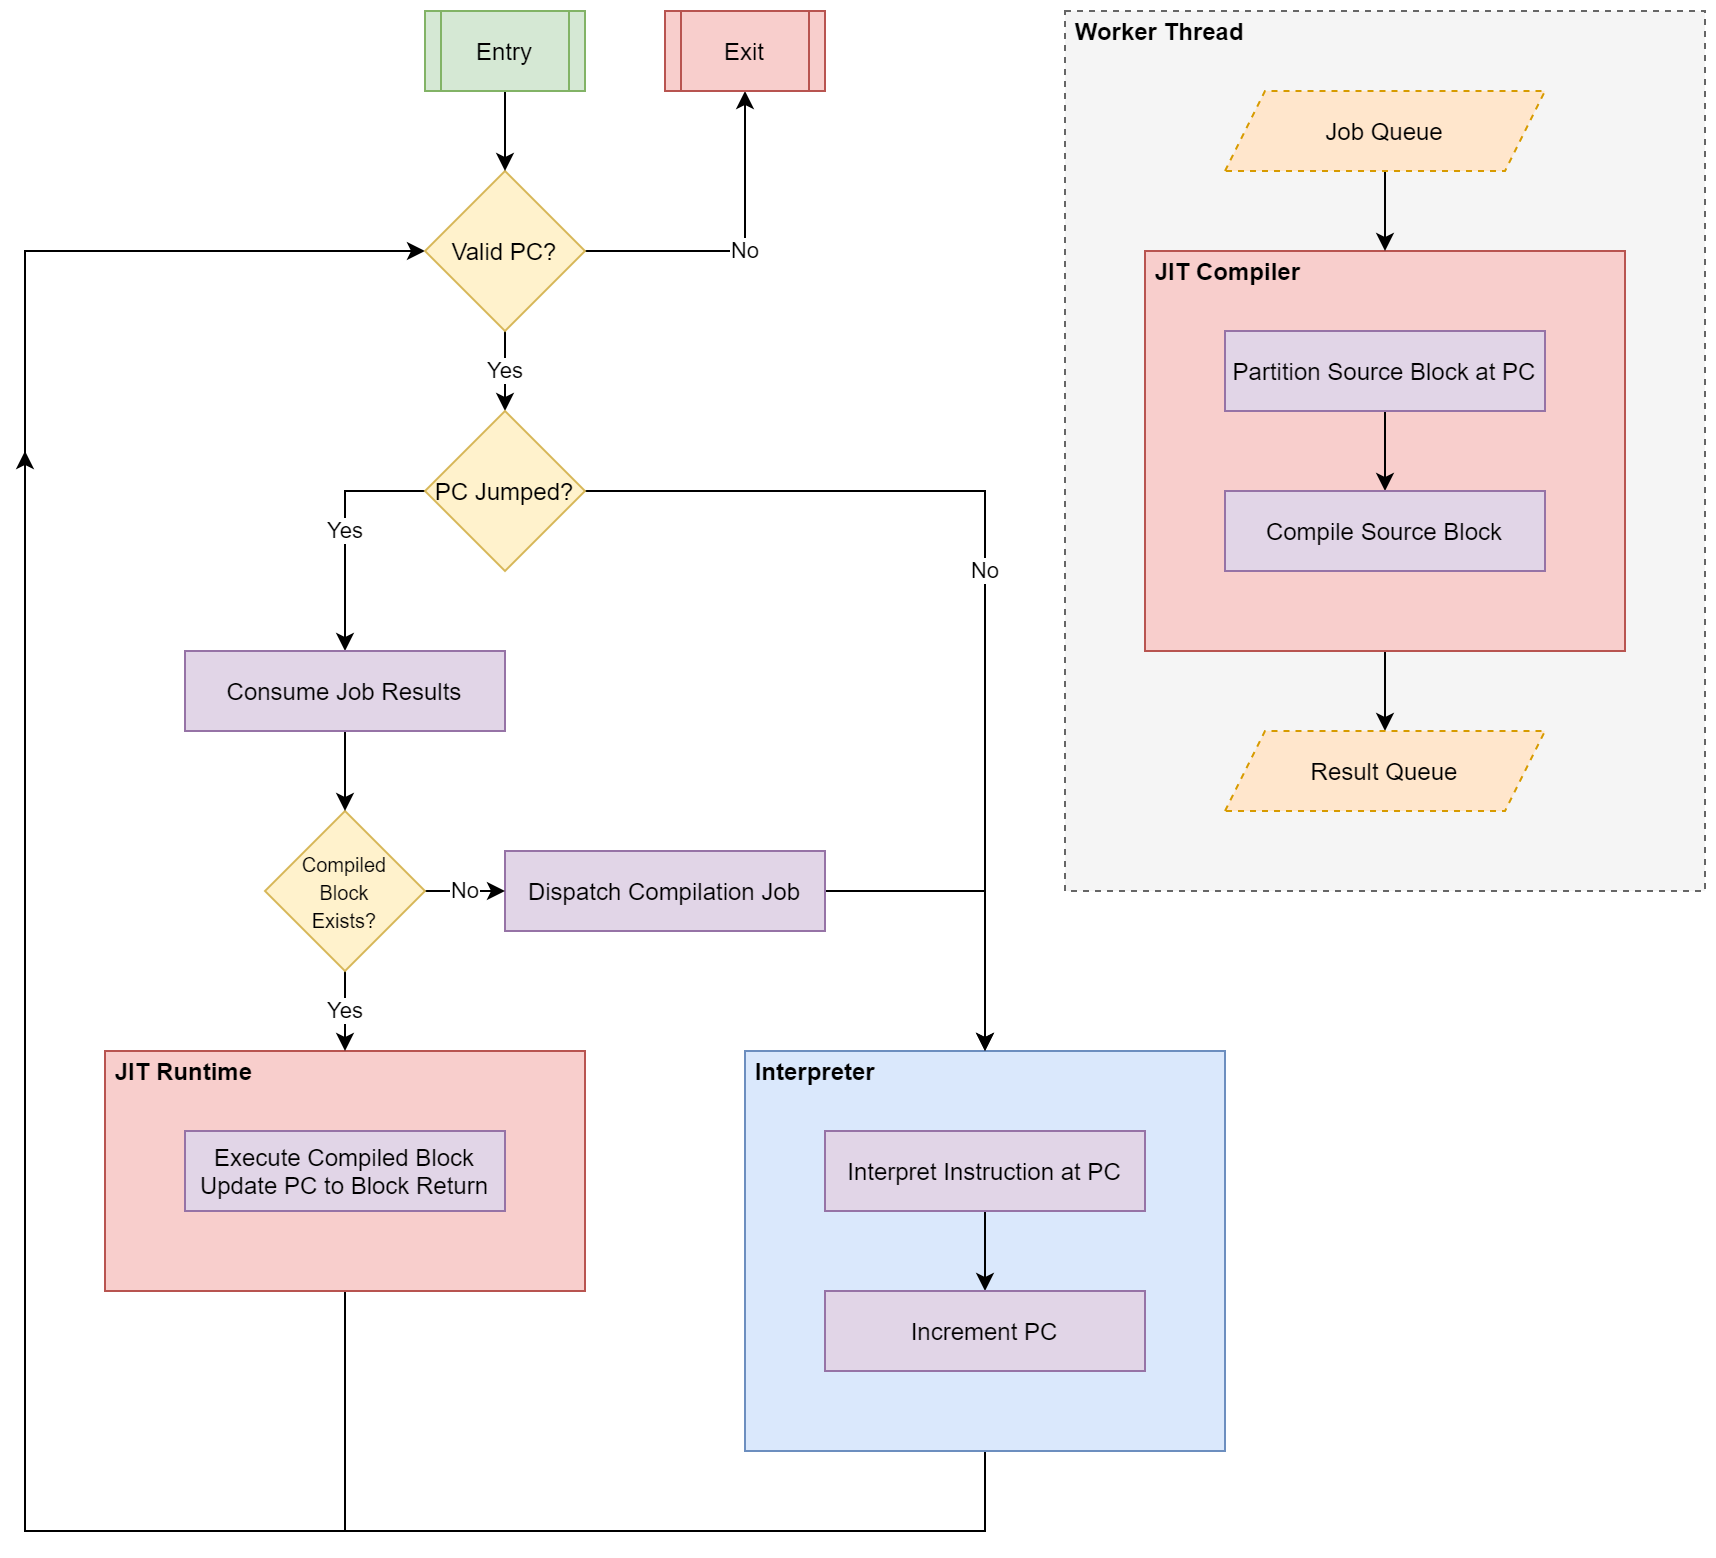
\includegraphics[width=1\linewidth]{diagrams/hybrid.png}
    \caption{Top level architecture of the hybrid emulator.}
    \label{figure:hybrid-arch}
\end{figure}

This combination allows it to defer the compilation of blocks to asynchronous worker threads, leaving the main thread free to emulate the program either via the JIT compiled blocks or the interpreter fallback. This minimizes the latency associated with JIT compilation as it is deferred into a non-blocking task. At the same time, the high execution performance of the JIT is \emph{eventually} present. This system can be expanded to multiple worker threads, allowing full utilization of the systems CPU for maximum compilation throughput.

The emulator contains a single state (memory map, register file etc.) that is shared between the interpreter and JIT components ensuring consistent behaviour no matter which means of emulation is used for any given block.

In some programs the compiler threads may be overloaded with compilation jobs being queued faster than they can be processed. Whilst not a disaster, this is non-ideal as very frequently executed blocks may be left in the queue for a long time due to the queue being filled with unimportant and infrequently used blocks. This would result in worse performance as the interpreter will be used more than necessary. To mitigate this, the compilation threshold denoted by \texttt{-T} is introduced. This threshold specifies how many times a block must be requested before it is actually compiled, ensuring that only sufficiently hot blocks are scheduled for compilation.